\begin{problem}{1.2}{problem1_2}

Repeat Exercise 1.1 approximating the \textit{sign} funcion in the control law by the sigmoid function $\text{sign}(\sigma) \approx \frac{\sigma}{|\sigma| + \varepsilon}$ and separately by the saturation function
\[
	\text{sign}(\sigma) \approx
	\begin{cases}
		1                          & \text{if } \quad \sigma > \varepsilon,       \\
		\frac{\sigma}{\varepsilon} & \text{if } \quad  |\sigma| \leq \varepsilon, \\
		-1                         & \text{if } \quad  \sigma < -\varepsilon.
	\end{cases}
\]

\end{problem}

\begin{solution}{}{solution1_2}
	As the analysis is practically the same as in Exercise 1.1, we will only show the results for the sigmoid and saturation approximations, and a discussion of the results.
	\begin{enumerate}[label=\textbf{\alph*)}, start=3]
		\item \begin{enumerate}[label=\textbf{\roman*)}]
			      \item Using the saturation approximation, we have:
			            \[
				            u = m(-c x_2 + v) = m \left( -c x_2 - \left( \rho + \frac{1.9}{m} x_2^2 \right) \text{sat}(\sigma) \right).
			            \]

			            \begin{figure}[H]
				            \centering
				            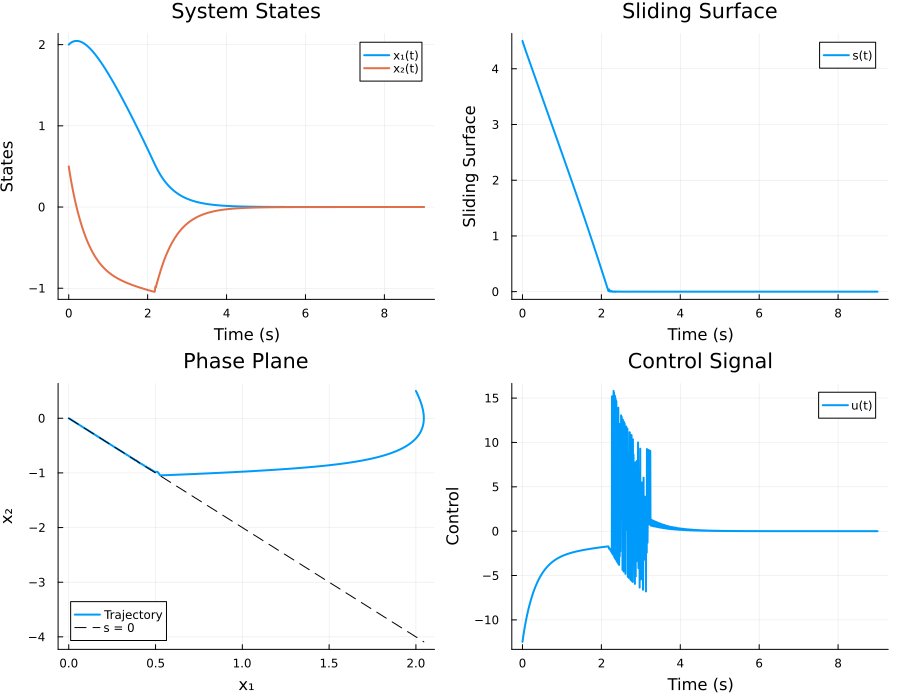
\includegraphics[width=1\textwidth]{img/problem1_2_sat.png}
				            \caption{Simulation results for the sliding mode control system using saturation approximation.}
				            \label{fig:problem1_2_sat}
			            \end{figure}

			      \item Using the sigmoid approximation, we have:
			            \[
				            u = m(-c x_2 + v) = m \left( -c x_2 - \left( \rho + \frac{1.9}{m} x_2^2 \right) \frac{\sigma}{|\sigma| + \varepsilon} \right).
			            \]

			            \begin{figure}[H]
				            \centering
				            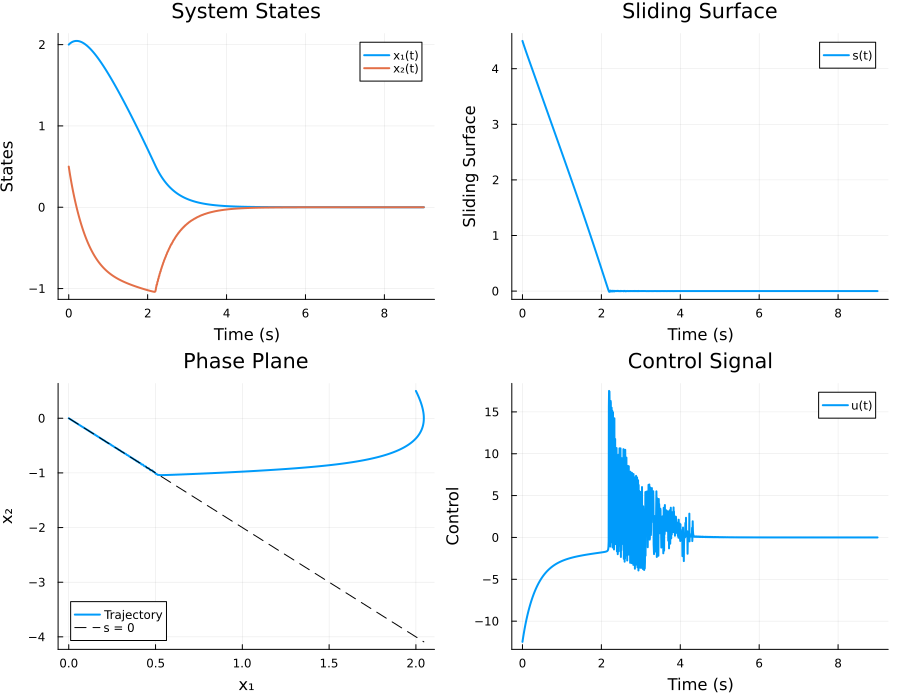
\includegraphics[width=1\textwidth]{img/problem1_2_sigmoid.png}
				            \caption{Simulation results for the sliding mode control system using sigmoid approximation.}
				            \label{fig:problem1_2_sig}
			            \end{figure}
		      \end{enumerate}
	\end{enumerate}
	In both cases, we can observe that the system seems to have finite time convergence in the sliding variable, and the chattering attenuation in the control input is evident. The saturation approximation leads to a more abrupt control action at the beginning, while the sigmoid approximation provides a smoother transition. Despite this, both approximations yield similar results in terms of system behavior and performance. It is clear that both approximations are effective in reducing chattering, but the theory suggests that both approximations only drive the sliding variable asymptotically to zero, so these are not ideal sliding modes, even though, in this case, and with that very small $\varepsilon$, the system behaves as if it were a sliding mode in both cases.
	\qed
\end{solution}